% XXX discuss the spill-in efficiency etc.

\documentclass[../thesis.tex]{subfiles}

\begin{document}

\chapter{Fitting}
\label{chap:fitting}

\section{Overview}
\label{sec:fitoverview}

% XXX show that we can neglect energy spread due to positron angular distribution. Where do E0 values for fastn shape come from? Add big tables of all rates and efficiencies (one per data period). Fix greek characters in Fig 8.4. Plot resolution function.

In order to extract neutrino oscillation parameters, Daya Bay data is compared to the predictions associated with different parameter values, and the extracted parameters are then those that give the best fit to the data. Given knowledge of the reactor \nuebar flux, detector response, and expected backgrounds, it is conceptually straightforward to generate a set of predictions. However, calculating the goodness of fit (while properly accounting for systematic and statistical uncertainties), and then assigning errors to the extracted parameters, is where the procedure becomes more subtle and complex. In Daya Bay, separate analysis groups have historically employed two different approaches, theoretically equivalent but implemented very differently. These are the method of pull terms (a.k.a. nuisance parameters), and the covariance matrix approach. In this analysis, we use the latter, but both will be briefly described in this introductory section. In the rest of this chapter, we detail the fitting machinery developed at LBNL \cite{berkeley_shapefit,berkeley_toymc}.

\subsection{Method of pull terms}
\label{sec:pullterms}

In the method using pull terms, the fitter is ``smart'' in the sense that it has knowledge of the various underlying models (reactor \nuebar flux, detector response, backgrounds, etc.) and knows how their predictions will change under changes of the systematic uncertainties. In this approach, each systematic is represented by a \emph{pull term} (or \emph{nuissance parameter}), which is in turn assigned an uncertainty of its own. An example of such a pull term might be the relative energy scale of a given AD. Each pull term is assigned a nominal value, corresponding to our best estimate given available knowledge. Then, during the fit, not only are the oscillation parameters varied, but so are the pull terms, and the predictions are transformed accordingly. The total $\chi^2$ then takes a form similar to
\begin{equation}
  \chi^2 = \sum_i \frac{(x_i - \widebar x_i)^2}{\sigma_i^2} + \sum_j \frac{(\eta_j - \widebar \eta_j)^2}{\varsigma_j^2},
\end{equation}
where $x_i$ are the measured data (e.g., AD spectra), $\widebar x_i$ are the predictions (which vary as we scan the oscillation parameters and pull terms), $\sigma_i$ are the \emph{statistical} uncertainties on the data, $\eta_j$ are the pull terms, $\widebar \eta_j$ are their nominal values, and $\varsigma_j$ are the uncertainties on the pulls.

Fitting is complete when the fitter has found the values of the oscillation parameters \emph{and pull terms} that minimize the total $\chi^2$. The 1$\sigma$ errors on the oscillation parameters are then based on the amount of variation required to increase the reduced\footnote{We use the term ``reduced $\chi^2$'' to refer to the $\chi^2$ divided by the number of degrees of freedom.} $\chi^2$ by 1 unit (or 2.3 for a 2D fit,\footnote{Based on the fact that $(1/2\pi)\int_{\theta=0}^{2\pi} \int_{r=0}^{r_0} e^{-r^2/2}\, r\,dr\,d\theta$ = 0.68 when $r_0 = 2.3$.} etc.), while minimizing over the pull terms at every step. Correlations between energy bins are handled implicitly; the information is encoded in how the predictions in different bins are shifted together when the pull terms are varied.

\begin{comment}
  See doc-8774 p29 and its ref 22 regarding the amount of chi2 increase for a 2D fit.
\end{comment}

\subsection{Covariance matrix approach}
\label{sec:covmatapproach}

As an alternative to using pull terms, uncertainties and correlations can be encoded in a single covariance matrix generated using Monte Carlo techniques. In this approach, the fitter is relatively ``dumb'': It knows only how to generate a prediction using a \emph{nominal} model (of, again, reactors, backgrounds, detectors, etc.) and how to vary the prediction for different values of the oscillation parameters. It has no idea how the prediction will transform under varying assumptions with respect to systematic uncertainties. (This knowedge belongs to the Monte Carlo.) The fitter's job is simply to take the measurements $x_i$, the predictions $\widebar x_i$ (which vary according to the oscillation parameters), and the covariance matrix $V_{ij}$, and then to find the oscillation parameters which minimize the $\chi^2$,
\begin{equation}
  \label{eq:fitCovChiSq}
  \chi^2 = (x_i - \widebar x_i) V_{ij}^{-1} (x_j - \widebar x_j).
\end{equation}
A major advantage of this approach is that it greatly reduces the dimensionality of the minimization---instead of minimizing over potentially dozens of pulls (as well as the oscillation parameters), only the two oscillation parameters must be considered. The computational cost and risk of falling into false minima are thus avoided. A disadvantage is the need to possibly take extra steps in order to ensure an invertible covariance matrix (see \autoref{sec:fitCombo}), and the need to carefully treat correlations, which are implicitly accounted for when using pull terms.

In the LBNL fitter, the full NuWa-based Monte Carlo is not used for generating the covariance matrix, due to its complexity and computational cost. Instead, a ``toy'' MC, described in \autoref{sec:toymc}, was developed for this purpose.

\subsection{Relative or absolute?}
\label{sec:fitRelOrAbs}

In addition to the choice between using pull terms or a covariance matrix (or some hybrid of the two), there is also the orthogonal option of performing a relative or an absolute fit. In a relative fit, the near-site data is used to generate predictions for the far sites, which are then compared to the far-site data. Whereas in an absolute fit, predictions are generated for both the near and the far sites, for comparison to both the near and far observations. The main advantage of performing a relative fit is that the absolute detection efficiency (both its nominal value and its uncertainty) can be ignored completely, since it has no bearing on the process of near-to-far extrapolation. On the other hand, a relative fit requires dealing with multiple correlated predictions and/or the merging of data between ADs, and implementing it in the context of a pull-term fitter is not as straightforward as doing an absolute fit. In any case, both approaches should ultimately give the same results. The LBNL fitter takes the relative approach, as discussed further in \autoref{sec:fitFitter}.

\section{Toy Monte Carlo}
\label{sec:toymc}

The primary purpose of the LBNL toy MC \cite{berkeley_toymc} is to enable the computation of the covariance matrix $V_{ij}$ in \autocite{eq:fitCovChiSq}. It does so by generating a large collection of simulated ``toy'' experiments, with each one represented by the prompt spectrum measured by each AD. The covariance matrix can then be derived from the variations within the collection, as detailed in \autoref{sec:fitToyOutputs}. Each toy experiment may include fluctuations due to statistics and/or a chosen set of systematics.\footnote{In practice, statistical fluctuations are disabled, since the statistical covariance matrix is calculated analytically as described in \autoref{sec:fitStatCovMat}.} As detailed later, a given systematic is incorporated by, first, describing it (analogously to a pull term) by a parameter (such as the detection efficiency), and then fluctuating the parameter; the value of the parameter is then used by the toy MC's model for generating the prompt spectra. This basic functionality enables the production of three essential inputs used by the fitter:

\begin{itemize}
\item The covariance matrices for signal and background systematics, used in calculating the $\chi^2$ during the fit. As will be explained, the signal covariance matrix is rescaled according to the signal size, and then added to the background covariance matrix to produce the full systematic matrix, which is finally added to the statistical covariance matrix (generated on the fly by the fitter).
\item The ``super histograms'': The nominal (i.e. unfluctuated) predicted cross section-weighted antineutrino spectrum produced by each core. This is used when breaking down the near-site spectra into reactor contributions for extrapolation to the far site.
\item The conversion matrix between prompt energy $\Erec$ and true antineutrino energy $\Enu$; this is also used in the extrapolation.
\end{itemize}

In addition, the toy MC provides a method of validating the fitter, since toys can be generated for any chosen values of $\tAC$ and $\Dmsqee$, thus enabling the testing of the fitter's ability to recover the same values.

\begin{comment}
  The toy MC also generates a ``PredictedIBD'' file which contains the background-free no-oscillation IBD spectra of each detector. As far as I can tell, this is only used in order to calculate a `summed' covariance matrix in which the matrices of the three stages (6, 8, 7AD) are combined, with the weighting determined by the PredictedIBD counts. (Oscillations shouldn't affect this weighting between ADs in the same hall, or the weighting between different stages.) In turn, the summed matrix is not used during the fit, but is only produced as a diagnostic. 
\end{comment}

\subsection{Binning}
\label{sec:fitBinning}

In the fitter and toy MC, two (somewhat arbitrary) options are available for the reconstructed energy binning:

\begin{enumerate}
\item ``LBNL'' binning: One bin from 0.7 to 1~MeV, 35 bins of 0.2~MeV from 1 to 8~MeV, and one bin from 8 to 12~MeV, for a total of 37 bins.
\item ``BCW'' binning: One bin from 0.7 to 1.3~MeV, 24 bins of 0.25~MeV from 1.3 to 7.3~MeV, and one bin from 7.3 to 12~MeV, for a total of 26 bins.
\end{enumerate}

The spectrum below 1.3~MeV is particularly susceptible to distortion from the IAV effect. In turn, if the IAV effect (\autoref{sec:fitIavEffect}) is imperfectly modeled, this can lead to a $\sim1\sigma$ bias in the extraction of $\Dmsqee$, as was indeed observed during comparisons of the results between the independent analysis groups. The use of a coarser binning at low energies thus removes any sensitivity to this distortion. For this reason, the BCW binning is preferred (at least pending improvements to the IAV matrix).

\subsection{IBD spectrum at each AD}
\label{sec:fitToyFluxPred}

The toy MC chain begins with the prediction of the livetime-averaged antineutrino spectrum $F_c(E_\nu)$ produced (per unit time) at each reactor core $c$, as specified by \autoref{eq:reacToyFinalPred}.\footnote{The technical details of this prediction are described in \autoref{sec:reactoy}, and the underlying theory is discussed in \autoref{chap:reactor}.} This is then used to calculate the IBD spectrum at each AD $i$ as
\begin{equation}
  \label{eq:fitTrueIbdSpec}
  R_i(E_\nu) = T_i\,N_i\,\epsilon_i\,\sigma(E_\nu) \sum_c F_c(E_\nu) \frac{1}{4\pi L_{ci}^2}
  \Posc(E_\nu, L_{ci})
\end{equation}
where $T_i$ is the livetime, $N_i$ is the number of target protons, and $L_{ci}$ is the baseline.

The detection efficiency $\epsilon_i$ includes the calculated efficiencies of the muon veto and the multiplicity cut (both of which are considered to have negligible uncertainty), as well as an additional factor which accounts for all of the remaining efficiency components. This factor is identical for all ADs in the nominal case, but when allowing fluctuations (as when generating toy samples for the construction of the covariance matrix), the efficiency is assigned an AD-to-AD uncorrelated uncertainty of 0.11\% $\oplus$ 0.072\% (\autoref{sec:miscDetEff}), with the latter component fully correlated with the variation in the energy scale of the AD.
% \footnote{The relative energy scale uncertainty is 0.2\%, as described later. Studies have shown \cite{P15A_inputs} that a 1\% energy scale variation leads to a 0.36\% shift in detection efficiency (largely due to the delayed energy cut), so we have 0.36 $\times$ 0.20\% $\sim$ 0.072\%.%
  % Also see doc-8027.
% }

The cross section $\sigma(E_\nu)$ is calculated by performing a $4\pi$ numerical integration of the differential cross section (to first order in the inverse nucleon mass $1/M$) \cite{Vogel_1999}. Letting $\theta$ be the angle between the antineutrino and the positron in the lab frame (with the proton initially at rest),
\begin{equation}
  \label{eq:ibdXsec}
  \frac{d\sigma}{d\cos\theta} = \frac{\sigma_0}{2}
  \left[\vphantom{\frac{\sigma_0}{2}}
    (f^2 + 3g^2) + (f^2 - g^2) v_e^{(1)} \cos\theta\right]
  E_e^{(1)} p_e^{(1)} 
  - \frac{\sigma_0}{2}
  \left[\frac{\Gamma}{M}\right]
  E_e^{(0)} p_e^{(0)}, 
\end{equation}
where
\begin{equation}
  \begin{aligned}
  \Gamma & =
  2 (f + f_2) g
  \left[ (2 E_e^{(0)} + \Delta ) ( 1 - v_e^{(0)}\cos\theta)
    -\frac{m_e^2}{E_e^{(0)}} \right] \\
  & +
  (f^2 + g^2)
  \left[ \Delta( 1 + v_e^{(0)}\cos\theta)
    + \frac{m_e^2}{E_e^{(0)}} \right] \\
  & + 
  (f^2 + 3g^2)
  \left[ (E_e^{(0)} + \Delta) (1 - \frac{1}{v_e^{(0)}}\cos\theta) - 
    \Delta\right] \\
  & +
  (f^2 - g^2)
  \left[ (E_e^{(0)} + \Delta) (1 - \frac{1}{v_e^{(0)}}\cos\theta) - 
    \Delta\right] v_e^{(0)} \cos\theta,
\end{aligned}
\end{equation}
and
\begin{align}
  \sigma_0 &= \frac{G_F^2 \cos^2\theta_C}{\pi}\; (1 + \Delta^R_{\mathrm{inner}}), \\
  \label{eq:firstOrderEnergy}
  E_e^{(1)} &= E_e^{(0)}
  \left[1 - \frac{E_{\nu}}{M}(1 - v_e^{(0)} \cos \theta) \right]
              - \frac{y^2}{M}, \\
  E_e^{(0)} &= E_\nu - \Delta, \\
  v_e^{(i)} &= \frac{p_e^{(i)}}{E_e^{(i)}}, \\
  \Delta &= M_n - M_p, \\
  M &= \frac{M_n + M_p}{2}, \\
  y^2 &= \frac{\Delta^2 - m_e^2}{2}.
\end{align}
The various constants that enter this cross section are taken from \cite{pdg2011} (unless noted otherwise) and summarized in \autoref{tab:xsecConstants}.\footnote{It is often stated (e.g., in \cite{spectrum2017}) that the cross section is calculated using the neutron lifetime $\tau_n$ from a particular edition of the PDG tables. However, $\tau_n$ can only be directly used when calculating $\sigma$ to zeroth-order in $1/M$ \cite{Vogel_1999}. In the first-order calculation \autoref{eq:ibdXsec}, $\tau_n$ does not appear explicitly. Nevertheless, other constants, such as $g$, are connected to $\tau_n$ and are thus modified by updated measurements of the latter.}

\begin{table}[ht]
  \begin{tabular}{llc}
    \toprule
    Symbol & Description & Value \\
    \midrule
    $G_F$ & Fermi coupling constant & $1.16637 \times 10^{-5}\; (\hbar c)^3$ GeV$^{-2}$ \\
    $\hbar c$ & Planck constant times speed of light & $197.3269631$ MeV fm \\
    $f$ & Vector coupling $g_V/g_V$ & 1 \\
    $g$ & Axial coupling $g_A/g_V$ & 1.2701 \\
    $f_2$ & Anomalous isovector magnetic moment $\mu_p - \mu_n$ & 3.70589 \\
    $\cos \theta_C$ & Cabbibo angle & 0.974 \\
    $\Delta^R_{\mathrm{inner}}$ & Inner radiative correction \cite{doi:10.1063/1.59543} & 0.024 \\
    $M_p$ & Proton mass & 938.272013 MeV \\
    $M_n$ & Neutron mass & 939.565345 MeV \\
    $m_e$ & Electron mass & 0.51099891 MeV \\
    \bottomrule
  \end{tabular}
  \caption{Constants used in the evaluation of \autoref{eq:ibdXsec} \cite{pdg2011}.}
  \label{tab:xsecConstants}
\end{table}

Returning to \autoref{eq:fitTrueIbdSpec}, $\Posc$ is calculated according to \autoref{eq:survProbDybFull}, which of course depends on the oscillation parameters.\footnote{By default, the toy MC assumes the normal hierarchy when using \autoref{eq:hierarchy} to convert $\Dmsqee$ into $\Delta m^2_{32}$ and $\Delta m^2_{31}$ for insertion into \autoref{eq:survProbDybFull}.} \autoref{tab:toyNomOscPars} summarizes the nominal oscillation parameters used in generating the covariance and response matrices.\footnote{In princple, full self-consistency would require regenerating the matrices after a fit (using the best-fit oscillation parameters), repeating the fit, and iterating this sequence until the results converge. However, in practice, the matrices do not vary significantly in the vicinity of the $\chi^2$ minimum, so this complication is unnecessary as long as the nominal parameters are reasonably close to the minimum.%
  % XXX is the matrix stable even out to the 3$\sigma$ contours?
}
Other values of the oscillation parameters can be used for benchmarking the fitter, e.g., verifying that it recovers the parameters used by the toy MC.

\begin{table}[ht]
  \begin{tabular}{lc}
    \toprule
    Parameter & Value \\
    \midrule
    $\SinSq$ & 0.084 \\
    $\Dmsqee$ & $2.48 \times 10^{-3}$ eV$^2$ \\
    $\sin^2 2\theta_{12}$ & 0.851 $\pm$ 0.021\\
    $\Delta m^2_{21}$ & (7.53 $\pm$ 0.18) $\times$ $10^{-5}$ eV$^2$ \\
    \bottomrule
  \end{tabular}
  \caption{Nominal oscillation parameters used by the toy Monte Carlo. For the solar parameters, the indicated errors are used for generating random fluctuations about the nominal values.}
  \label{tab:toyNomOscPars}
\end{table}

\subsection{Detector response}
\label{sec:fitToyDetResponse}

Once the toy MC has determined each AD's IBD spectrum (in terms of the antineutrino energy), the next step is to convert it into a prompt-energy spectrum. This entails four steps:

\begin{enumerate}
\item Converting antineutrino energy into positron energy
\item Accounting for the ``loss'' of visible energy incurred when positrons deposit some of their energy in the acrylic wall of the IAV
\item Converting scintillator-deposited energy into mean visible energy, according to the absolute energy scale and the nonlinearity model
\item Smearing the visible energy according to the resolution of the AD
\end{enumerate}

\subsubsection{Positron energy}

As with the IBD cross section discussed previously, the positron energy is calculated to first order in the inverse nucleon mass scale $1/M$. \autoref{eq:firstOrderEnergy} gives the first-order positron energy $E_e^{(1)}$ as a function of the lab-frame antineutrino-positron angle $\theta$. Meanwhile, the mean value of $\cos\theta$, weighted by the differential cross section \autoref{eq:ibdXsec}, is \cite{Vogel_1999}
% Since \autoref{eq:firstOrderEnergy} depends linearly on $\cos \theta$, the mean positron energy can then be obtained by replacement in \autoref{eq:firstOrderEnergy} of $\cos\theta$ with $\langle \cos \theta \rangle$, the mean value (weighted by the differential cross section \autoref{eq:ibdXsec}) of $\cos \theta$. Computing this mean gives \cite{Vogel_1999}
\begin{equation}
  \label{eq:meanIbdAngle}
  \langle \cos \theta \rangle = -0.034\, v_e^{(0)} + 2.4 \frac{E_\nu}{M}.
\end{equation}
Since $E_e^{(1)}$ is a linear function of $\cos\theta$, the mean positron energy is then simply obtained by inserting $\langle \cos\theta \rangle$ into \autoref{eq:firstOrderEnergy} in place of $\cos\theta$:
\begin{equation}
  \label{eq:firstOrderEnergyMean}
  \langle E_e^{(1)} \rangle = E_e^{(0)}
  \left\{1 - \frac{E_{\nu}}{M}\left[1 - v_e^{(0)} \left(-0.034\, v_e^{(0)} + 2.4 \frac{E_\nu}{M}\right)\right] \right\}
  - \frac{y^2}{M},
\end{equation}
where $E_e^{(0)}$, $M$, etc.\@ were defined in \autoref{sec:fitToyFluxPred}.

Later, in \autoref{sec:fitResolution}, we show that it is safe to neglect the energy spread caused by the angular distribution, as it is negligible in comparison to the dominant factors in the energy resolution (primarily photon statistics, as well as detector nonuniformity and noise). Likewise, there is no need to extend the calculation to higher order, given that the neutron carries away only $\mathcal{O}$(10~keV) of kinetic energy.

\subsubsection{IAV effect}
\label{sec:fitIavEffect}

\newcommand\Miav{\mathbf{M}^{\mathrm{IAV}}}
\newcommand\Eetrue[1]{E^{\mathrm{true}}_{e#1}}
\newcommand\Eels[1]{E^{\mathrm{LS}}_{e#1}}

For IBDs that occur near the edge of the inner acrylic vessel, some of the positron's kinetic energy may be deposited in the acrylic, rendering that energy invisible.\footnote{Some of the energy from the annihilation gammas can also disappear in this way. The Daya Bay MC accounts for this.} In order to model this effect, it was simulated in the full Daya Bay MC \cite{TruePromptSpec}, producing a matrix $\Miav_{ij}$ which converts ``true'' positron energy $\Eetrue{}$ into ``LS-deposited'' positron energy $\Eels{}$,
\begin{equation}
  \label{eq:Miav}
  \Eels{,i} = \Miav_{ij} \Eetrue{,j}
\end{equation}
where $i$ and $j$ are bin indices, and $\Miav$ is subject to the normalization condition $\sum_i\Miav_{ij} = 1$ for all true energy bins $j$ (i.e., the conversion preserves the total antineutrino count, as it should). Each axis of $\Miav$ contains 240 bins of width 50~keV ranging from 0 to 12~MeV.

The uncertainty of the IAV wall thickness is assigned a conservative 4\%, which is assumed to translate to a 4\% uncertainty on the elements of $\Miav$. As implemented, the matrix is fluctuated by applying an independent 4\% Gaussian variation to each off-diagonal element, and then setting the diagonal elements so as to restore the normalization condition.

\subsubsection{Positron to mean reconstructed energy}

As discussed in \autoref{sec:reconEnergyNL}, the reconstructed energy is affected by nonlinearity in the scintillator (quenching, Cerenkov radiation) and in the electronics. Our analysis makes use of the ``unified'' nonlinearity model described in \cite{EnergyModelUpdateYongbo}.
% Within the Daya Bay collaboration, a great deal of widespread effort went toward characterizing this behavior, as described in \cite{NonlinearityPaper}. The sum of this work was distilled in April 2018 by Yongbo Huang \cite{EnergyModelUpdateYongbo} to produce a ``unified'' nonlinearity model for use in analysis. This model is used in the toy MC.
The unified nonlinearity model takes the form of a nominal curve (tabulating the ratio of reconstructed to positron energy, as a function of positron energy), along with four pull curves (\cite{EnergyModelUpdateSoeren}, p10) that express the uncertainty in the model. The nominal curve and the $\pm68\%$ CL bands were shown in \autoref{fig:reconPositronNominal}. All curves (nominal and pulls) were generating using the full Daya Bay MC, as controlled by five parameters (absolute energy scale, Birks/Cerenkov constants, electronics parameters). The curve that best fit a collection of source/$^{12}$B data was designated the nominal curve. Meanwhile, among 250 random curves within 68\% CL, the pull curves were taken as the four that best spanned the remaining 246. The four pulls thus account for the correlations inherent in the shape uncertainty, without requiring the use of a full covariance matrix during analysis. \autoref{fig:nonlinPullCurves} shows the nominal curve along with the four pulls. The model parameters for these five curves were never published, and cannot easily be recovered from a fit (since the Cerenkov nonlinearity function $f_c$ was tabulated numerically and was also never published). Instead, the author and other Daya Bay analyzers were simply provided with tabulated values of the five curves for use in analysis.

\begin{figure}[ht]
  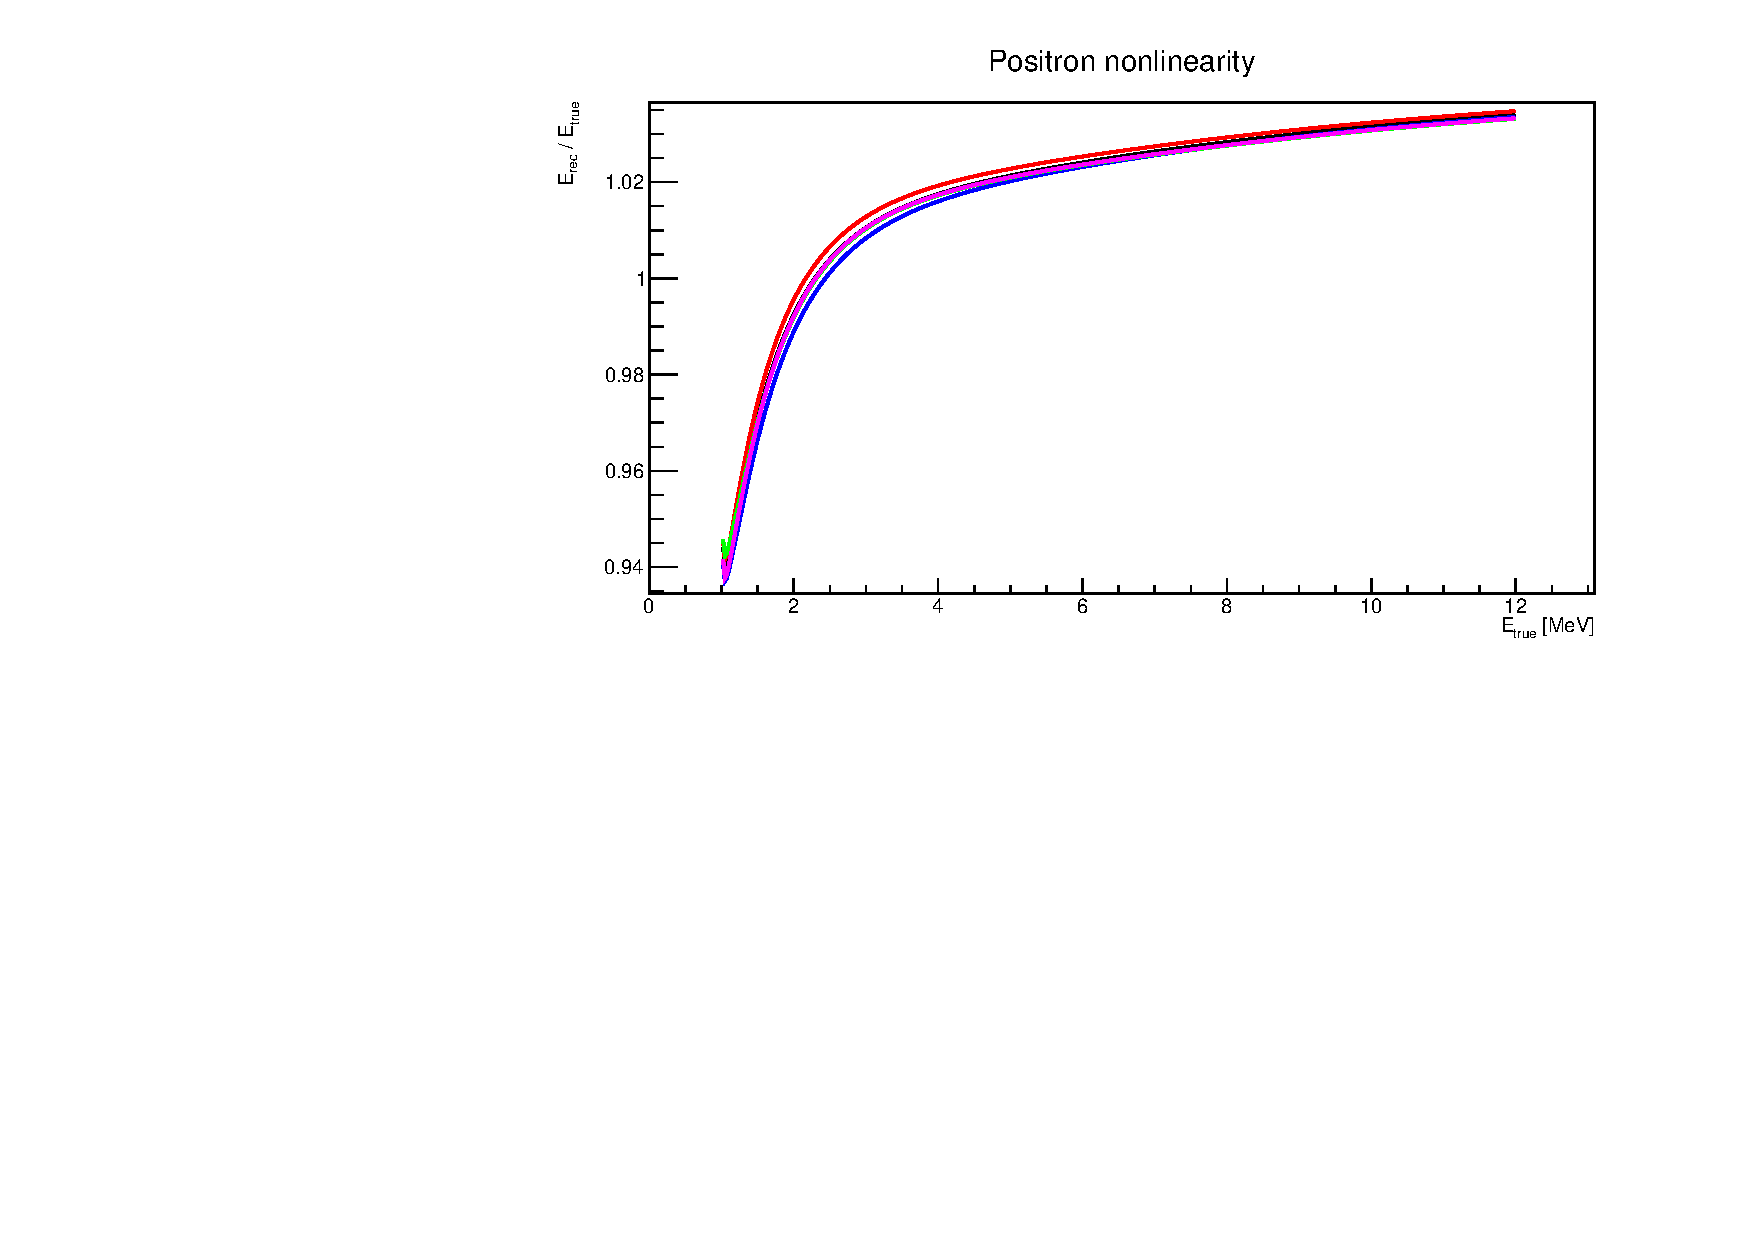
\includegraphics[width=\textwidth]{Fitting/eplusNLpulls.pdf}
  \caption{The nominal curve (black) from the unified nonlinearity model, along with the four pull curves (red, blue, magenta, green). The green curve only differs noticeably from the nominal curve at the lowest energies.}
  \label{fig:nonlinPullCurves}
\end{figure}
% XXX should show pulls minus nominals

Based on the unified model, a nonlinearity curve is generated according to
\begin{equation}
  \label{eq:fitRandomNL}
  f_{\mathrm{ran}}(E_e) = f_{\mathrm{nom}}(E_e) + \sum_p^4 a_p [ f_p(E_e) - f_{\mathrm{nom}}(E_e)],
\end{equation}
where $E_e$ is the positron energy, and the $a_p$ are standard Gaussian random variables. (We will continue using $a$ to denote such variables.) The same curve is used in all detectors. However, where the ADs \textit{can} differ is in their overall energy scales. The relative energy scale uncertainty has been estimated to be 0.2\% \cite{berkeley_shapefit_P14A}. Accordingly, for each toy, and each AD $d$, a scaling factor $k_d$ is calculated as
\begin{equation}
  k_d = 1 + a_d \cdot 0.002.
\end{equation}
The final relationship between the positron and reconstructed energy, for AD $d$, is then
\begin{equation}
  \Erec = F_d(E_e) = k_d \cdot f_{\mathrm{ran}}(E_e) \cdot E_e.
\end{equation}

Using this relationship, the number of events $N_{\mathrm{rec},i}$ in the $i$th bin of reconstructed energy (centered at $E_{\mathrm{rec},i}$) is calculated as
\begin{equation}
  \label{eq:fitNrec}
  N_{\mathrm{rec},i}(E_{\mathrm{rec},i}) = N_{e,j} \left( \frac{dF}{dE_e} \Bigr|_{E_{e,j}} \right)^{-1} \frac{\Delta_{\mathrm{rec}}}{\Delta_{\mathrm{e}}}
\end{equation}
where the index $j$ is such that
\begin{equation}
  F(E_{e,j}) = E_{\mathrm{rec},i},
\end{equation}
and the $\Delta$ are the bin widths.

\subsubsection{Detector resolution}
\label{sec:fitResolution}

As described in \cite{An_2017}, the Daya Bay detector resolution has been characterized as taking the form
\begin{equation}
  \label{eq:resolution}
  \frac{\sigma(E_{\mathrm{rec}})}{E_{\mathrm{rec}}} = \sqrt{(1.6\%)^2 + \frac{(8.1\%)^2}{E_{\mathrm{rec}}}
    + \frac{(2.6\%)^2}{E_{\mathrm{rec}}^2}},
\end{equation}
where the three terms correspond to detector nonuniformity, photoelectron statistics, and noise, respectively. In \autoref{fig:energyReso} we plot this function, along with its uncertainty bands (discussed later). The coefficients were determined by performing a fit to the gamma-ray peaks from various calibration sources and neutron captures, as well as to the alpha-particle peaks from radioactivity \cite{An_2017}. This model does not account for the intrinsic energy spread of the IBD positron due to its angular distribution. We proceed to justify this omission, first heuristically and then quantitatively.

\begin{figure}[ht]
  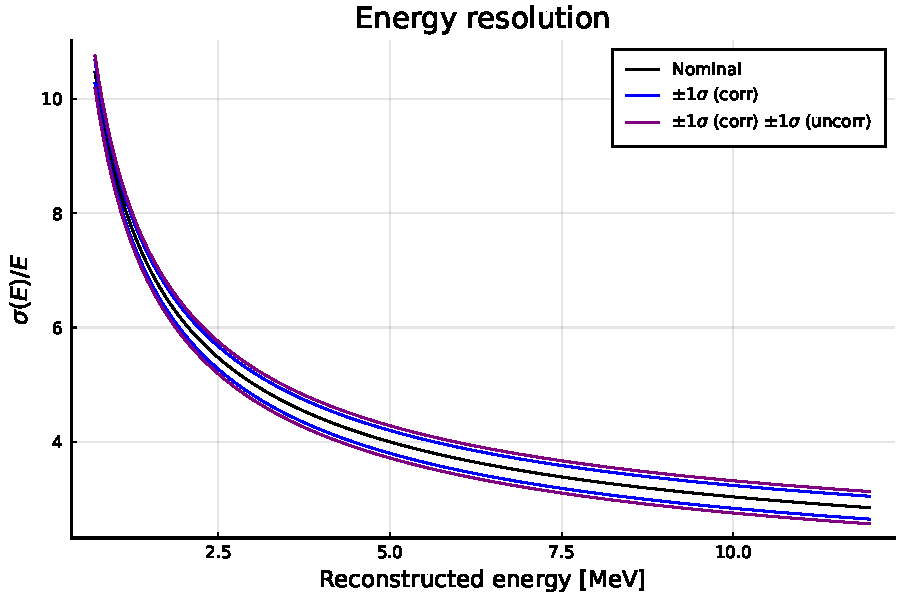
\includegraphics[width=0.7\textwidth]{Fitting/energyReso.pdf}
  \caption{The energy resolution model (\autoref{eq:resolution}) and its uncertainty bands (AD-correlated and total).}
  \label{fig:energyReso}
\end{figure}

From \autoref{eq:firstOrderEnergy}, it can be seen that the first-order angular dependence of the positron energy takes the form
\begin{equation}
  \delta E = E_e^{(0)} \frac{E_\nu}{M}v_e^{(0)}\cos\theta.
\end{equation}
We aim to determine the worst-case energy spread, so we may conservatively let $v_e^{(0)} = 1$. Now, for the highest antineutrino energy observed at Daya Bay, around 9~MeV, we have $E_\nu/M \approx 1\%$. Then, since $\cos\theta$ ranges from -1 to 1, we have
\begin{equation}
  \frac{\max(\delta E) - \min(\delta E)}{E_e^{(0)}} \approx 2\% \left( \frac{E_\nu}{\SI{9}{MeV}} \right).
\end{equation}
That is, the \emph{total spread} of the positron energies is, in the worst case ($E_\nu = \SI{9}{MeV}$), 2\%, and gets linearly smaller for lower antineutrino energies. Translating this 2\% total spread into a standard deviation, for comparison with the resolution model, requires knowledge of the shape of the energy distribution. As we show later, however, this distribution is reasonably flat, so for the sake of this qualitative argument, we will assume a uniform energy distribution. For a uniform distribution of total spread $S$, the standard deviation $\sigma$ is given by\footnote{In what follows, $\sigma$ (without a derivative symbol) will always refer to a standard deviation, while cross-sections will always be treated in differential form, $d\sigma$, thus avoiding any ambiguity.}
\begin{equation}
  \sigma = \frac{S}{2\sqrt{3}}.
\end{equation}
For the positron energy distribution, this gives
\begin{equation}
  \begin{aligned}
    \sigma & \approx \frac{2\%}{2\sqrt{3}} \left( \frac{E_\nu}{\SI{9}{MeV}} \right) \\
    & = 0.6\% \left( \frac{E_\nu}{\SI{9}{MeV}} \right).
  \end{aligned}
\end{equation}
The question now is whether this kinematic energy spread is significant in comparison to the modeled energy resolution in \autoref{eq:resolution}. From \autoref{fig:energyReso} it is clear that we need only consider the highest-energy case, since at lower energies, the fractional kinematic spread gets smaller while the modeled resolution gets larger. According to \autoref{fig:energyReso}, the modeled resolution levels off at around 4\%. Adding the 0.6\% kinematic spread in quadrature then increases the total resolution to 4.05\%. Thus, heuristically, the effect is negligible.

To address the issue more rigorously, we can directly calculate the standard deviation of the positron energy by using the differential cross-section (\autoref{eq:ibdXsec}) and the relation between the first-order energy $E_e^{(1)}$ and the scattering angle (\autoref{eq:firstOrderEnergy}). In \autoref{fig:positronAnglePDF}, we normalize $d\sigma/d\cos\theta$ to obtain the probability distribution function (PDF) of $\cos\theta$, plotted for various values of the antineutrino energy $E_\nu$. The PDFs are relatively flat, as was claimed earlier, with a modest bias toward backscattering. In order to visualize the energy spread that arises from the angular distribution, in \autoref{fig:positronDEvsAngle} we plot the \emph{positron energy deficit} $E_\nu - E_e^{(1)}$ (i.e., the amount of energy transferred to the hadronic system) as a function of $\cos\theta$ for various values of $E_\nu$. All of the curves approximately intersect in the forward-scattering limit, where the neutron kinetic energy is minimal and the deficit is approximately the neutron-proton mass difference of 1.29~MeV. As expected, the deficit increases for harder scattering angles and higher $E_\nu$ as more kinetic energy is transferred to the neutron. For the case of $E_\nu = \SI{9}{MeV}$, the difference between the maximum and minimum $E_e^{(1)}$ is 0.15~MeV. Relative to $E_e^{(1)}$ ($\approx E_\nu - 1.3 = \SI{7.7}{MeV}$), the size of this spread is 1.9\%, consistent with the 2\% we estimated earlier.

\begin{figure}[ht]
  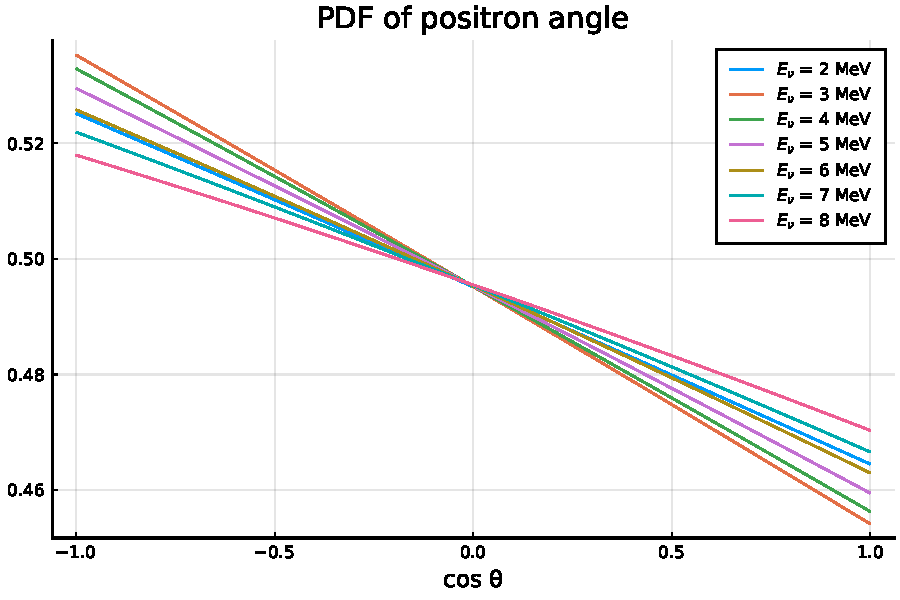
\includegraphics[width=0.7\textwidth]{Fitting/positron_angle_pdf.pdf}
  \caption{Probability distribution functions of the scattering angle for IBD positrons.}
  \label{fig:positronAnglePDF}
\end{figure}

\begin{figure}[ht]
  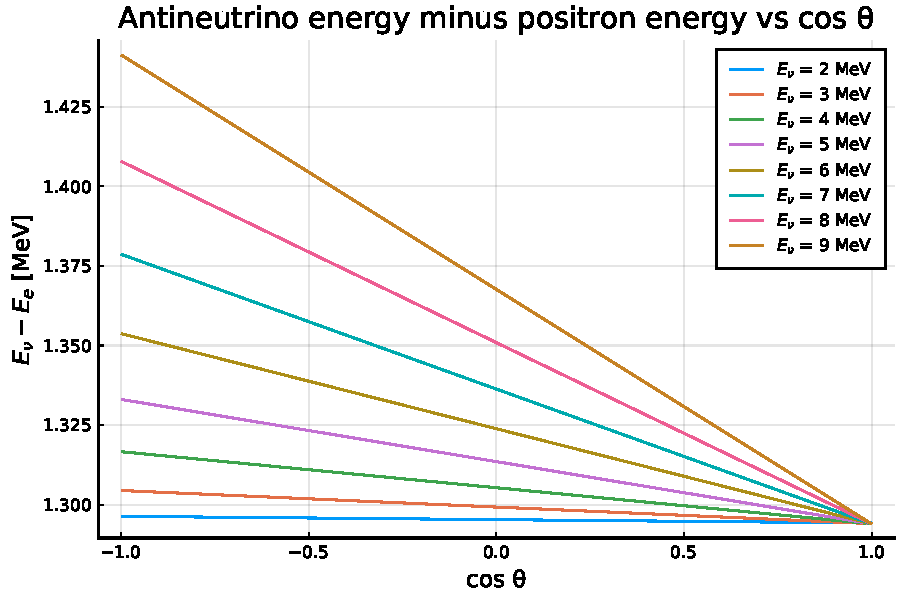
\includegraphics[width=0.7\textwidth]{Fitting/positron_energyDiff_vs_angle.pdf}
  \caption{Dependence of the positron energy deficit (i.e. the amount of energy transferred to the hadronic system) on the scattering angle.}
  \label{fig:positronDEvsAngle}
\end{figure}

To go further and directly calculate the standard deviation of the positron energy, we require the PDF of the latter, which can be obtained by normalizing the energy-differential cross-section
\begin{equation}
  \frac{d\sigma}{dE_e^{(1)}} = \frac{d\sigma}{d\cos\theta} \left( \frac{dE_e^{(1)}}{d\cos\theta} \right)^{-1},
\end{equation}
where the derivative $dE_e^{(1)}/d\cos\theta$ is evaluated at the angle $\theta'$ corresponding to energy $E_e^{(1)}$. Operationally, we determine $\theta'$ by numerically inverting \autoref{eq:firstOrderEnergy}. In \autoref{fig:positronEnergyDiffPDF} we plot the PDFs (for various values of $E_\nu$) as a function of the \emph{percent deviation of the positron energy from the mean} (where the mean is individually computed for each value of $E_\nu$). As was claimed earlier, these distributions are relatively flat. As expected, they are broader for higher values of $E_\nu$, and there is a slight bias toward lower energies (i.e.\  backscattering).

\begin{figure}[ht]
  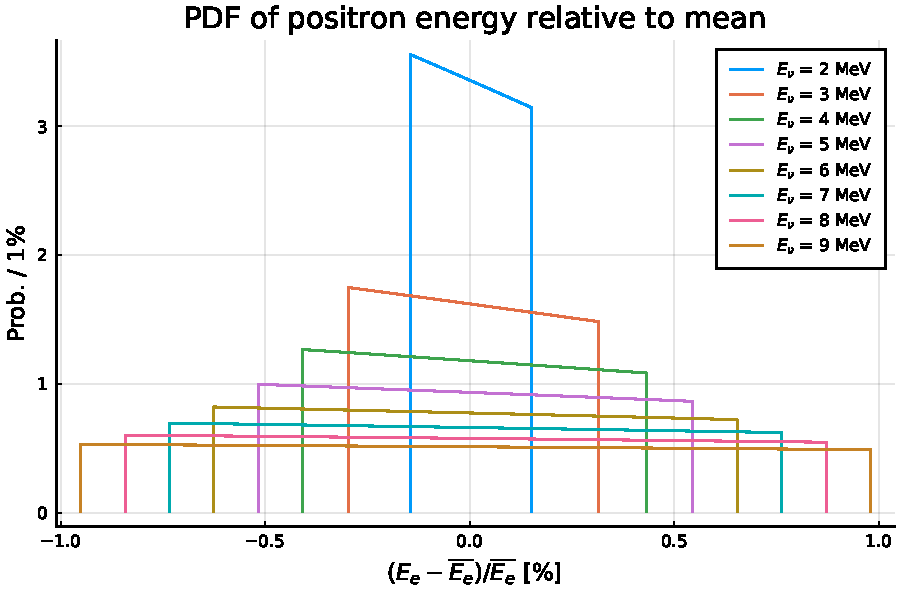
\includegraphics[width=0.7\textwidth]{Fitting/positron_relEnergy_pdf.pdf}
  \caption{Probability distribution functions of the positron energy (expressed as percentage deviations from the mean energy for fixed $E_\nu$).}
  \label{fig:positronEnergyDiffPDF}
\end{figure}

At this point, all that remains is to take the standard deviations $\sigma$ of these energy PDFs. The resulting values are in percentage terms, which can be directly compared to the modeled resolution (\autoref{eq:resolution} and \autoref{fig:energyReso}) in order to determine the significance of this energy spread. In fig \autoref{fig:positronSpreadPct}, we plot this $\sigma$ as a function of $E_\nu$. The results are in excellent agreement with our previous estimate: In the worst case (at 9~MeV), $\sigma$ is only about 0.6\%. As was argued earlier, this is insignificant relative to the energy resolution model.\footnote{Since some of the reconstructed energy comes from the annihilation electron, which is not subject to this spread, this analysis overestimates the size of the effect, further highlighting its insignificance.}

\begin{figure}[ht]
  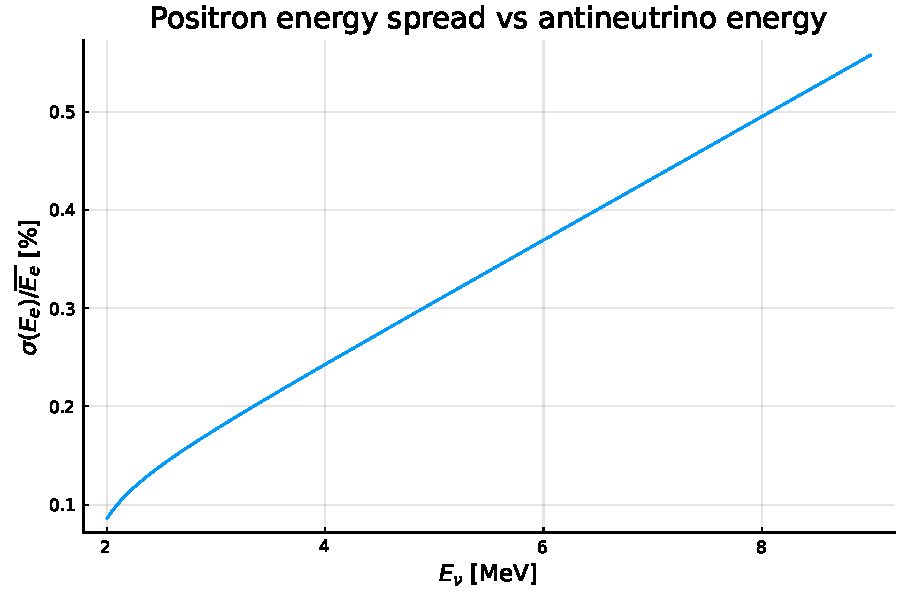
\includegraphics[width=0.7\textwidth]{Fitting/positron_spread_pct.pdf}
  \caption{Standard deviation of the positron energy (due to its angular distribution) as a function of antineutrino energy.}
  \label{fig:positronSpreadPct}
\end{figure}

In the official Daya Bay publications (e.g., \cite{An_2017}), the uncertainty of the resolution has been declared to be negligible. However, we apply the conservative uncertainties originally employed by the LBNL analysis: 0.2\% correlated and 0.2\% uncorrelated. The correlated component is due to the statistical uncertainty of the (old) resolution fits (with limited statistics), while the uncorrelated part is attributed to the observed 0.2\% AD-to-AD differences in the reconstructed energy \cite{berkeley_toymc}. Resolution fluctuations are applied as a constant shift to the fractional uncertainty. As such, for detector $d$, $\sigma/E_{\mathrm{rec}}$ is fluctuated according to
\begin{equation}
  \frac{\sigma_{\mathrm{ran},d}(E_{\mathrm{rec}})}{E_{\mathrm{rec}}} = \frac{\sigma(E_{\mathrm{rec}})}{E_{\mathrm{rec}}} + (0.2\% \times a_{\mathrm{corr}})  + (0.2\% \times a_d).
\end{equation}

Application of the detector resolution begins with the ``source'' $\Erec$ histogram produced according to \autoref{eq:fitNrec}. An identically-shaped (but empty) ``destination'' histogram is then constructed, and for each destination bin centered at $E_{\mathrm{rec},i}$, we loop over the ``source'' bins that span $E_{\mathrm{rec}i} \pm 8\,\sigma(E_{\mathrm{rec},i})$,\footnote{8 standard deviations was chosen in order to ensure ``almost all'' relevant events would be included. In practice, 4 or 5 standard deviations would have been more than sufficient.} and increase the count in the destination bin by the contents of the source bin, times the appropriate Gaussian factor. This produces the final, smeared, IBD spectrum.

\subsection{Backgrounds}
\label{sec:fitToyBackgrounds}

The toy MC's treatment of backgrounds is based on the discussion in \autoref{chap:bkg}. Here we briefly review the determination of the rate and shape (and their respective uncertainties) of each background. Fluctuations may be applied differently for different backgrounds; for instance, for some backgrounds each AD is fluctuated independently, while for others the fluctuations are correlated. Such details will also be covered in what follows. In all cases, the rate and shape uncertainties are decoupled; that is, shape fluctuations are implemented by distorting the spectrum and then renormalizing it to its previous integral, while rate fluctuations involve uniformly scaling all bins by the same factor.

\subsubsection{Accidentals}

The accidental-background rate is calculated from data per \autoref{sec:accratecalc}, and the shape is likewise extracted from data as described in \autoref{sec:selSingles} and \autoref{sec:singsel}. The statistical uncertainty of the accidentals rate is dominated by the $\sim$0.2\% ($\sim$0.4\%) near (far) uncertainty in the delayed-like singles rate. (In \autoref{sec:accStatUnc}, we obtain a consistent total uncertainty in the accidentals rate using a simple Monte Carlo). However, the calculated accidentals rate could be systematically biased by low-energy correlated processes (e.g. $\alpha$-$\alpha$). To study this possibility, studies within the collaboration cross-checked the accidental-rate measurement using samples of artificial accidentals obtained by requiring an additional time offset between the prompt and delayed triggers \cite{An_2017}. These gave rates that were consistent with the standard calculation, up to the 1\% statistical uncertainty of the cross checks. This 1\% is thus conservatively defined to be the uncertainty of the accidentals rate.

Rate fluctuations are applied independently for each AD. No shape uncertainty is assigned, given the substantial statistics of the background sample and the fact that the uncertainty in each energy bin is more than covered by the overall rate uncertainty.
% (XXX should show that the shape doesn't vary much for different isolation cuts.)

\subsubsection{\LiHe}

The calculation of the \LiHe\ rate is described in \autoref{sec:bkgCosmo}, as is the prediction of the spectrum, which assumes a 5.5\% proportion of $^8$He. Given the limited statistics of the $^9$Li sample, it is not possible to measure statistically significant differences in the $^9$Li rate within a given hall. Accordingly, all ADs in a hall are treated identically. Rate fluctuations are thus applied to each \emph{hall} independently. In order to enable fluctuation of the shape, a sample of 250 random \LiHe\ spectra were produced under 100\% variations of the alpha-particle and neutron quenching factors. (The $^8$He proportion was not varied during this process, since its impact is small compared to that of the quenching factors.) For each fluctuated toy sample, a spectrum is chosen at random from this set. The same random spectrum is used among all ADs.

\subsubsection{Fast neutrons}

The fast neutron rate and shape were estimated using a number of techniques, as described in \autoref{sec:bkgFastn}. As with \LiHe, rate fluctuations are applied on a per-hall basis. The nominal shapes take the form of \autoref{eq:bkgFastnShape}, with the parameter $E_0$ specified for each hall, and $a$ fixed to be zero.\footnote{As noted in \autoref{sec:fastn_extrap}, it has been shown that there is no significant effect from allowing a nonzero $a$ when fitting \autoref{eq:bkgFastnShape} to the fast-neutron spectrum \cite{fastn}.} based on fits to data samples enriched in fast neutrons. For shape fluctuations, the key consideration is the fact that most of the shape uncertainty lies at low energies. Accordingly, for each toy sample, we first generate a Gaussian random variable $k$:
\begin{equation}
  k = \Gaus(0,1),
\end{equation}
and then an empirical distortion factor is generated:
\begin{equation}
  y(E) = k \cdot E^{-0.1} + c,
\end{equation}
where $c$ is determined such that that $y = 1$ (i.e. no distortion) at 12~MeV:
\begin{equation}
  c = 1 - k \cdot E^{-0.1}.
\end{equation}
When $k = \pm1$, the size of this distortion is 25\% at 0.7~MeV. The distorted shape is obtained by multiplying the nominal spectrum by $y(E)$. The same distorted spectrum is used for all ADs.

\subsubsection{AmC}

As described in \autoref{sec:bkgAmC}, the AmC rates and a nominal measured spectrum from the high-activity AmC source (HAS) were obtained from studies within the collaboration \cite{AmC_paper}. The ensuing uncertainty was deemed to be dominated by potential biases in the procedure itself (i.e. MC simulations and measurement of a high-activity source), rather than by statistics or AD-to-AD variations. As such, both rate and shape fluctuations are applied consistently among all ADs. The nominal spectrum was obtained by fitting the HAS spectrum to an exponential according to \autoref{eq:amc_fit_func}. Shape fluctuations are then implemented by varying the exponential's slope by $\pm$0.15\%, based on the recommendation of studies internal to the collaboration.

\subsubsection{$\CanO$}

The rate and its uncertainty for the $\CanO$ background are described in \autoref{sec:bkgCanO}. Rate fluctuations are applied independently among all ADs. No shape fluctuations are applied, since this background is very small and the rate uncertainty is very conservative.

\subsection{Outputs}
\label{sec:fitToyOutputs}

\subsubsection{``Super histograms''}

The so-called \emph{super histograms} $S_c$ are essentially the cross section-weighted antineutrino spectra produced by each core, with some arbitrary (but consistent) normalization:
\begin{equation}
  S_c(E_\nu) \propto \sigma(E_\nu)\,F_c(E_\nu).
\end{equation}
The calculation of the cross section $\sigma(E_\nu)$ is described in \autoref{sec:fitToyFluxPred}, and the core spectrum $F_c(E_\nu)$ is given by \autoref{eq:reacToyFinalPred}. As an implementation detail, these histograms are calculated in the toy MC by applying \autoref{eq:fitTrueIbdSpec} for a single core, with all of the AD-specific quantities (baseline, etc.) set to unity (or an arbitrary constant), and $\theta_{13}$ set to zero (likewise for $\theta_{12}$). The super histograms are used to calculate the fraction of each AD's spectrum that is attributable to each core, as needed when extrapolating near-site measurements to the far site. The normalization is unimportant, since only the ratios matter in this calculation.

\subsubsection{Reverse response matrix}

In the fitter (\autoref{sec:fitFitter}), we require a ``reverse response'' matrix $\mathbf{M}$ to convert the prompt energy to the antineutrino energy for extrapolation to the far site. This matrix is generated as a two-dimensional ROOT histogram, in which the $x$ axis represents antineutrino energy in 240 bins from 0 to 12~MeV, and the $y$ axis represents prompt energy (in either the LBNL or BCW binning).\footnote{In our mathematical treatment here, we ``flip'' the axes in accordance with the normal convention for matrices: For an element $\mathbf{M}_{ij}$, the ``vertical'' index $i$ refers to a particular antineutrino energy (the ``output''), and the ``horizontal'' index $j$ refers to a particular reconstructed energy (the ``input''). It is merely a historical implementation detail that the ROOT histogram uses the opposite convention.}

\begin{comment}
  I don't see any reason to mention the fact that a finer binning (2880 instead of 240) is used internally by the toy MC when generating this matrix. With the standard 240 bins, the edges line up with both the LBNL and BCW edges, so there shouldn't be any benefit from using a finer binning.

  deleted: Internally, the toy MC normally represents both neutrino and prompt energy using 240 bins (of 50~keV) from 0 to 12~MeV.
\end{comment}

For the near-to-far extrapolation, we require the ability to convert from $\Erec$ to $E_\nu$. However, the toy MC can only go in the opposite direction, from $E_\nu$ to $\Erec$. We could thus easily produce a ``forward'' response matrix $\mathbf{M_{fwd}}$ by looping over $E_\nu$ bins and populating their columns with the corresponding (normalized) $\Erec$ spectra. The result could then be trivially used for converting $E_\nu$ to $\Erec$:
\begin{equation}
  \mathbf{S_{rec}} = \mathbf{M_{fwd}} \mathbf{S_\nu} 
\end{equation}
where the $\mathbf{S}$ are the spectra.\footnote{\label{foot:fitEnuToErec}In practice, the fitter does not use this method to convert $E_\nu$ to $\Erec$ at the end of the extrapolation. Instead, a separate $E_\nu$ spectrum is extrapolated for each $\Erec$ bin, and the result is then integrated back into the original $\Erec$ bin. This method is perhaps not quite as rigorous, but there is no evidence of any resulting bias as long as the binning is sufficiently fine, as is the case for both the LBNL and BCW binnings.} Unfortunately, this matrix would not be directly invertible, greatly complicating the reverse transformation that we need. Meanwhile, use of the transpose, as in
\begin{equation}
  \mathbf{S_\nu} = \mathbf{M_{fwd}^{T}} \mathbf{S_{rec}},
\end{equation}
would only be valid if the antineutrino spectrum were flat, which is obviously not the case.

The solution to these difficulties is to reweight the $\Erec$ spectrum in each $E_\nu$ column of $\mathbf{M_{fwd}}$ according to the expected shape (in $E_\nu$) of the IBD spectrum.
% , and then take the transpose.
% This effectively gives a prediction of the 2D joint distribution of $E_\nu$ and $\Erec$.
Each \emph{row} of this $\mathbf{M_{fwd}^{reweight}}$ (corresponding to an $\Erec$ bin) can then be normalized to give an $E_\nu$ spectrum for each $\Erec$ bin. Under the assumption that the measured spectrum reasonably matches this shape, it is then valid to use the (transposed) result for converting an $\Erec$ bin to an $E_\nu$ distribution.

\begin{comment}
\footnote{Given that the shape is distorted both by oscillations and by differences in the fission fractions, it is important to verify that the analysis is insensitive to such variations in the spectral shape. XXX, was this done?}
\end{comment}

\begin{comment}
  We should fix genEvisToEnuMatrix.C to turn off the theta13 oscillation, and then note below that oscillations are disabled.
\end{comment}

Accordingly, to construct the reverse response matrix, the toy MC first generates a nominal antineutrino energy spectrum $\mathbf{S^{nom}_\nu}$ (for the arbitrary case of AD1). Backgrounds are not included, since the fitter subtracts them before converting $\Erec$ to $E_\nu$. The toy MC then loops over the 240 antineutrino energy bins. For each antineutrino energy bin $i$ (centered about $E_{\nu,i}$), it produces the corresponding PDF $f(\Erec; E_{\nu,i})$ of reconstructed energy (assuming a flat distribution of antineutrino energies within bin $i$), then scales it by the value of $\mathbf{S}^{\mathbf{nom}}_{\mathbf{\nu},i}$; the result is then assigned to the $i$th row of the matrix. Finally, each column of the matrix is normalized to unity:
\begin{align}
  \label{eq:revRespMtxUnNorm}
  \mathbf{M}^{\textbf{un-norm}}_{ij} &= \mathbf{S}^{\mathbf{nom}}_{\mathbf{\nu},i} \; f(E_{\mathrm{rec},j}; E_{\nu,i}), \\
  \label{eq:revRespMtx}
  \mathbf{M}_{ij} &= \frac{\mathbf{M}^{\textbf{un-norm}}_{ij}}{\sum_{j'=0}^{240} \mathbf{M}^{\textbf{un-norm}}_{ij'}}.
\end{align}

\subsubsection{Covariance matrices}

The covariance matrix, which encodes the scale of fluctuations between the far-site data and the prediction from the near sites (including correlations between ADs and energy bins), can be decomposed as the sum of three components, corresponding to signal (antineutrino) systematics, background systematics, and statistics. The statistical covariance matrix is calculated analytically by the fitter, as described in \autoref{sec:fitStatCovMat}. The two matrices for the systematics are generated by the toy MC, as detailed here.

Although the toy MC is capable of simultaneously varying the signal and background systematics, the two categories are treated separately due to differences in their scaling behaviors: The signal uncertainties scale with the size of the signal (which depends on the oscillation parameters), while the background uncertainties are constant.

To generate the covariance matrix for the signal systematics, a sample of $M =$~1,000 toy experiments is generated, using the nominal values of $\SinSq$ and $\Dmsqee$ from \autoref{tab:toyNomOscPars}, subject to the following fluctuations:

\begin{itemize}
\item Solar oscillation parameters (fluctuated according to the uncertainties listed in \autoref{tab:toyNomOscPars})
\item Reactor power (0.5\%, core-to-core uncorrelated)
\item Fission fractions (uncorrelated), isotope $\nubar$ spectra, non-equilibrium corrections, and spent fuel contributions (all correlated), as encapsulated by the covariance matrix from \cite{Lewis} (see \autoref{sec:reacunccorr})
\item IAV thickness (4\%, AD-to-AD uncorrelated)
\item Nonlinearity model, fluctuated according to \autoref{eq:fitRandomNL} (correlated)
\item Relative energy scale (0.2\%, uncorrelated)
\item Energy resolution (0.2\%, correlated $\oplus$ 0.2\%, uncorrelated). The two parts are treated as \emph{absolute} shifts to the (relative) resolution, and combined additively: $\sigma/E = \sigma_{\mathrm{nominal}}/E + \Gaus_1(0, 0.002) + \Gaus_2(0, 0.002)$.
\end{itemize}

From this sample of $M$ toy experiments, a ``normalized'' signal covariance matrix is constructed according to
\begin{equation}
  \label{eq:covmatSigNorm}
  (V^{\mathrm{norm}}_{\mathrm{sig}})_{ij} = \frac{1}{M} \sum_t^{M}
  \frac{(F^{\mathrm{obs},t}_i - F^{\mathrm{pred},t}_i)(F^{\mathrm{obs},t}_j - F^{\mathrm{pred},t}_j)}%
       {F^{\mathrm{pred},t}_i \cdot F^{\mathrm{pred},t}_j}
\end{equation}
Here, $F^{\mathrm{obs}}$ is the observed far-site data (after background subtraction), and $F^{\mathrm{pred}}$ is the predicted far-site data, as given by \autoref{eq:FPred}, based on the near-site observations. The denominator carries out the normalization, enabling the matrix to be rescaled according to the size of the signal in data, as described next. The indices $i$ and $j$ can potentially\footnote{Depending on how data is combined among ADs, as described in \autoref{sec:fitCombo}.} span (a) far ADs, (b) the near site(s)/AD(s) used for the prediction, (c) energy bins, and (d) data periods with different detector configurations. When the fitter calculates the $\chi^2$ at a given set of oscillation parameters, it rescales $(V^{\mathrm{norm}}_{\mathrm{sis}})_{ij}$ according to the predicted signal at the far site:
\begin{equation}
  (V_{\mathrm{sig}})_{ij} = (V^{\mathrm{norm}}_{\mathrm{sig}})_{ij} \cdot F^{\mathrm{pred}}_i(\SinSq, \Dmsqee)
  \cdot F^{\mathrm{pred}}_j(\SinSq, \Dmsqee).
\end{equation}
This uniform scaling procedure does not account for second-order variations in the ``shape'' of the covariance matrix as the oscillation parameters vary, but this simplification was found to have a negligible affect on the fit, so long as the assumed nominal parameters are reasonable.

For the background systematics, another set of $M = $ 1,000 toy experiments is generated (again with nominal oscillation parameters), subject to the rate and shape fluctuations described in \autoref{sec:fitToyBackgrounds}. From this sample the covariance matrix is calculated as
\begin{equation}
  \label{eq:covmatBG}
  (V_{\mathrm{bkg}})_{ij} = \frac{1}{M} \sum_t^{M}
  (F^{\mathrm{obs},t}_i - F^{\mathrm{pred},t}_i)(F^{\mathrm{obs},t}_j - F^{\mathrm{pred},t}_j)
\end{equation}
Note that this matrix is not ``normalized'' (i.e., there is no denominator, unlike in \autoref{eq:covmatSigNorm}), and thus there is no need to rescale it (i.e., multiply it by $F^{\mathrm{pred}}$). This difference in treatment between the signal and background matrices is due to the fact that the backgrounds (and hence their uncertainties) do not vary as a function of the oscillation parameters, while the converse is true for the signal.

\subsection{Handling of multiple data periods}
\label{sec:fitToyPeriods}

Some additional complexity arises from the fact that Daya Bay has operated under three different detector configurations: First with 6 ADs (missing EH2-AD2 and EH3-AD4), then with all 8, and finally with 7 (after the repurposing of EH1-AD1 for the JUNO experiment R\&D). In principle, the data from the three periods could simply be merged together. However, as explained in \autoref{sec:fitCombo}, obtaining an invertible covariance matrix requires combining data from ADs in the same sites, and this procedure is the simplest to implement when the (active) ADs have the same livetime, since they can be weighted equally. For this reason, the LBNL toy MC and fitter treat the three data periods as separate experiments (thus increasing the dimensionality of the prediction/observation vectors and the covariance matrix). However, some systematic fluctuations must be correlated among the periods, given that the overall experimental setup was the same (aside from some missing ADs). These correlations are summarized in \autoref{tab:fitToyPeriodCorr}.

\begin{table}[h]
  \centering
  \begin{tabular}[h]{lcc}
    \toprule
    & \multicolumn{2}{c}{Correlation between:} \\
    Fluctuated systematic & Detector & Period \\
    \midrule
    Relative efficiency/response & & \checkmark \\
    Solar parameters, nonlinearity & \checkmark & \checkmark \\
    Correlated background shapes & \checkmark & \checkmark \\
    Accidentals rates & & \\
    Fast-neutron and \LiHe\ rates & \checkmark (same hall) & \checkmark \\
    AmC rates & & \checkmark \\
    $\CanO$ rates & & \\
    \bottomrule
  \end{tabular}
  \caption{Correlations of systematics across detectors and periods. Reproduced from \cite{berkeley_shapefit_P14A}.}
  \label{tab:fitToyPeriodCorr}
\end{table}

\section{Fitter}
\label{sec:fitFitter}

Fundamentally, the task of the fitter \cite{berkeley_shapefit} is simply to find the oscillation parameters that best fit the observed data, where the quality of the fit is given by
\begin{equation}
  \chi^2 = \sum_{i,j} (\Fobs_i - \Fpred_i) V^{-1}_{ij} (\Fobs_j - \Fpred_j),
\end{equation}
with the total covariance matrix $V$ defined as
\begin{equation}
  V = V_{\mathrm{sig}} + V_{\mathrm{bkg}} + V_{\mathrm{stat}}.
\end{equation}
$V_{\mathrm{sig}}$ and $V_{\mathrm{bkg}}$ were described in \autoref{sec:fitToyOutputs}, while $V_{\mathrm{stat}}$ is described below in \autoref{sec:fitStatCovMat}. The indices $i$ and $j$ can run over detectors (or halls), energy bins, and data periods (6, 8, 7AD), depending on how the data (and covariance matrix) is merged across detectors, as described later. The main distinguishing characteristic of the LBNL fitter is that it takes a \emph{relative} approach: Rather than simultaneously fitting the near-site and far-site data directly, the near-site data is used to generate a far-site prediction, which is then compared to the data. The chief advantage of such an approach is that the absolute detection efficiency, shared among all ADs, cancels automatically, and therefore the covariance matrix can be generated without considering fluctuations in the absolute efficiency. Indeed, we could even ignore reactor uncertainties that are correlated among all cores, but because the reactor covariance matrix was designed to be useful for both relative and absolute fitters, they are accounted for anyway, unnecessarily but harmlessly.

The bulk of the fitter's complexity lies in the determination of the far-site prediction $\Fpred$ based on the near-site data, as well as in the aforementioned merging of data and the corresponding reduction of the covariance matrix.\footnote{This merging is necessary in order to obtain an invertible covariance matrix, given the high degree of correlation in the full covariance matrix.} In what follows we detail the steps taken by the fitter to ultimately determine the $\chi^2$ for a given set of oscillation parameters. Given the ability to calculate this $\chi^2$, finding the best fit can be done using standard minimization techniques, and a map of the $\chi^2$ across parameter space can be used to generate two-dimensional contours at any desired confidence level.

\begin{comment}
Compared to the toy Monte Carlo, the LBNL shape fitter is a relatively simple thing.

Its job is just to find the oscillation parameters that best fit the data, i.e. that give the lowest chi2.

It also produces a map of chi2 in parameter space for derivation of contours.
\end{comment}

\subsection{Far-site prediction from near sites}
\label{sec:fitNearToFarPred}

As was mentioned, the far-site data is predicted based on the measurements at the near sites. If Daya Bay were measuring antineutrinos from a single reactor, then this prediction could take place without any reference to reactor power and fission fraction data, resulting in a truly pure relative measurement. In reality, however, each near AD samples the flux from multiple reactors at different locations, which must each be treated individually when extrapolating to the far site. As such, reactor operational information must be used to decompose each near-site measurement into the components from each core. This process of near-to-far extrapolation, as implemented, essentially treats each bin of $\Erec$ as a separate subexperiment. For a single near AD, a single far AD, and a single $\Erec$ bin, the extrapolation proceeds as follows:

\begin{enumerate}
\item The reverse response matrix $\mathbf{M}$ from \autoref{eq:revRespMtx} is used to generate a distribution of $\Enu$, by taking the row corresponding to the $\Erec$ bin being extrapolated.
\item For each bin of $\Enu$, the contribution from each core is determined via \autoref{eq:fitFluxFactor} below, based on the predicted flux (according to power, fission fractions, and isotope spectra), the baselines, and the oscillation parameters.
\item For a single core's contribution to a single $\Enu$ bin, the extrapolation factor of \autoref{eq:fitExtrapFactor} is applied to obtain the predicted contribution at the far AD.
\item This is repeated for all cores, over all bins of $\Enu$, to generate a predicted $\Enu$ spectrum at the far AD \emph{for the single bin of $\Erec$ in question}.
\item The $\Enu$ spectrum is integrated back into the original $\Erec$ bin.
\end{enumerate}

This process is illustrated by \autoref{fig:fitExtrapCartoon}, and further details are given in the next section. After repeating this procedure for each $\Erec$ bin, a predicted prompt spectrum is thereby obtained at the far AD. Given that there are four near ADs and four far ADs (when all 8 ADs are operating), this results in a total of 16 predictions for each $\Erec$ bin. The 6AD and 7AD periods are essentially considered separate experiments (whose correlations due to systematics are encoded in the covariance matrix, as described in \autoref{sec:fitToyPeriods}), with 9 and 12 predictions for each $\Erec$ bin, respectively.

\begin{figure}[ht]
  \centering
  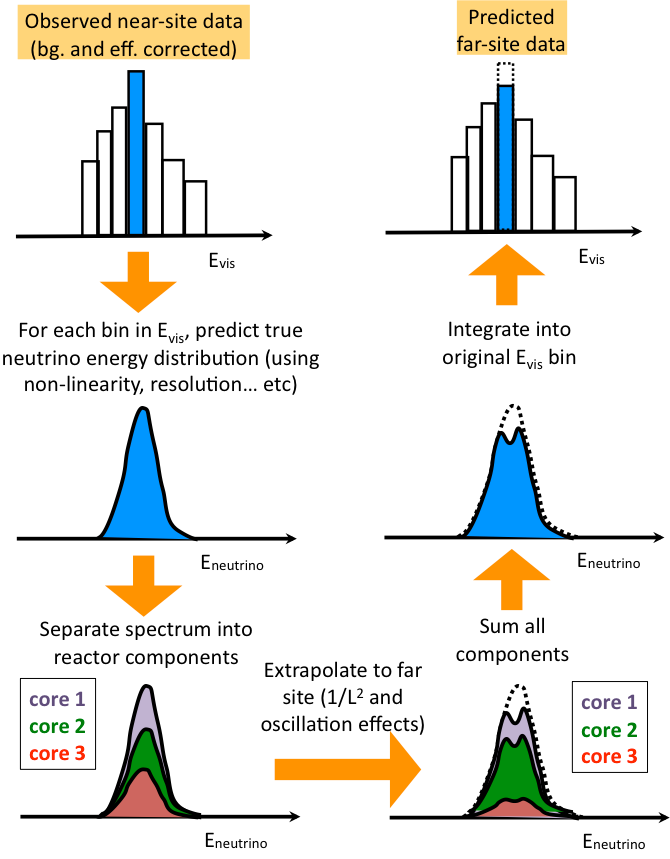
\includegraphics[scale=0.5]{extrap_cartoon.png}
  \caption{Conceptual illustration of the procedure for extrapolating a near AD measurement to a far AD. In the bottom-right panel, the dashed curve represents the unoscillated prediction. From \cite{berkeley_shapefit}.}
  \label{fig:fitExtrapCartoon} 
\end{figure}

\subsubsection{Mathematical details}

For a near AD $i$ and a given antineutrino energy $\Enu$, the fraction of the flux coming from core $k$ is given by the flux factor
\begin{equation}
  \label{eq:fitFluxFactor}
  f_{ik}(\Enu) = \frac{F_k(\Enu) \times P^{\mathrm{osc}}_{ik}(\Enu) \times 1/L^2_{ik}}
  {\sum_c F_c(\Enu) \times P^{\mathrm{osc}}_{ic}(\Enu) \times 1/L^2_{ic}},
\end{equation}
where $F_c(\Enu)$ is the antineutrino flux from core $c$, given by \autoref{eq:reacToyFinalPred}, and $L_{ic}$ is the baseline from core $c$ to AD $i$.

The observation at near AD $i$, attributable to core $k$, in true-energy bin $\Enu$, for the extrapolation of reconstructed-energy bin $\Erec$, is then simply
\begin{equation}
  N_{ik}(\Enu; \Erec) = f_{ik}(\Enu) \times N_i(\Enu; \Erec)
\end{equation}
where $N_i(\Enu; \Erec)$ is the background-subtracted count in the $\Enu$ bin:
\begin{equation}
  N_i(\Enu; \Erec) = \mathbf{M}(\Erec, \Enu) \times N_i(\Erec),
\end{equation}
and $N_i(\Erec)$ is the (background-subtracted) number of observed events in reconstructed-energy bin $\Erec$. For clarity, here we express the reverse response matrix $\mathbf{M}$ (from \autoref{eq:revRespMtx}) as a function of $\Erec$ and $\Enu$ rather than of bin indices.

In order to take near AD $i$'s observation of core $k$ and calculate the predicted observation at far AD $j$, we use the extrapolation factor
\begin{equation}
  \label{eq:fitExtrapFactor}
  e_{ij,k}(\Enu) = \frac{P^{\mathrm{osc}}_{jk}(\Enu) \times 1/L^2_{jk}}
  {P^{\mathrm{osc}}_{ik}(\Enu) \times 1/L^2_{ik}},
\end{equation}
which essentially removes the effects of baseline and oscillation from the near observation, and then applies them for the case of the far detector.

We then have the predicted flux contribution at the far AD:
\begin{equation}
  F^{\mathrm{pred}}_{ij,k}(\Enu; \Erec) = e_{ij,k}(\Enu) \times N_{ik}(\Enu)
\end{equation}

Then to get the final prediction at far AD $j$ from near AD $i$, we sum over all cores $k$ and integrate all $\Enu$ bins into the original $\Erec$ bin:
\begin{equation}
  \label{eq:FPred}
  F^{\mathrm{pred}}_{ij}(\Erec) = \sum_k \sum_{\Enu} F_{ij,k}(\Enu; \Erec)
\end{equation}

\begin{comment}
Near site spectrum divided into Erec bins.

For each bin, convert to true energy using matrix.

For each true energy bin (from this single Erec bin), determine fraction from each core using baselines and power.

For each core, undo 1/L^2 and oscillation, then apply them for each far site

Sum up cores, repeat for all Etrue bins (still for this single Erec bin)

Integrate back into original Erec bin at far site. Repeat for all bins.

In this way we get 16 predictions.
\end{comment}

\subsection{Statistical covariance matrix}
\label{sec:fitStatCovMat}

The near-to-far extrapolation produces multiple predictions for each far AD, one per near AD. Likewise, each near AD furnishes multiple predictions, one per far AD. Accordingly, statistical fluctuations in the near and far AD data will produce correlated fluctuations (across multiple near/far pairs) in the deviation between prediction and measurement. These correlations are encoded in the statistical covariance matrix, of which we describe the calculation here.

Technically speaking, fluctuations in the near-site data will produce fluctuations in $\Fpred$, while fluctuations in the far-site data will produce fluctuations in $\Fobs$. However, for the sake of simplicity, we choose to ``transfer'' the uncertainty on $\Fobs$ over to $\Fpred$, essentially leaving $\Fobs$ without any error bar. This simplifies the conceptual description of the covariance matrix (in the context of calculating $\chi^2$): It encodes fluctuations in $\Fpred$ around the ``fixed'' $\Fobs$. Of course, in reality, both quantities will fluctuate, but since it is only the \emph{difference} between the two that enters the $\chi^2$ calculation, we are free to divide the uncertainty between them as we please.

Given this convention, the statistical uncertainty on $\Fpred$ that arises from the near-site fluctuations is
\begin{equation}
  \snear(\Fpred) = \frac{\Fpred}{N^{\mathrm{obs}}} \sqrt{N^{\mathrm{obs}} + N^{\mathrm{bkg}}},
\end{equation}
where $N^{\mathrm{obs}}$ is the background-subtracted observation at the near AD, and $N^{\mathrm{bkg}}$ is likewise the predicted near AD background. In other words, this is the statistical uncertainty of the (background-subtracted) near measurement, scaled by the expected far-to-near ratio.

Meanwhile, the ``transferred'' statistical uncertainty on $\Fpred$ from far site fluctuations is simply
\begin{equation}
  \sfar(\Fpred) = \sqrt{\Fpred + F^{\mathrm{bkg}}},
\end{equation}
where $F^{\mathrm{bkg}}$ is the predicted background at the far AD. The total uncertainty on $\Fpred$ is then the sum of $\snear$ and $\sfar$, in quadrature.

As was noted, statistical correlations exist between pairs of predictions that share a near or far AD. It can be shown
% (XXX how???)
that, for two predictions (in the same $\Erec$ bin and data period) that arise from the same near AD, the covariance is the product of the two values of $\snear$. Similarly, for two predictions at the same far AD, the covariance is the product of the $\sfar$ values. And, of course, there is no covariance between different energy bins, data periods, or predictions that don't share a common AD. Based on the discussion thus far, it is then a simple matter to fill in the statistical covariance matrix. The tedious details depend on the way that the data is merged between ADs and on the technical definition of the indices $i$ and $j$; the code can be seen at \cite[ShapeFit/Predictor.C, Calculate(NearSite)StatError]{DybBerkFit}. Unlike the systematic components of the covariance matrix (which are fixed throughout the fit procedure, aside from rescaling), the statistical component is recalculated at each point in the parameter space.

\begin{comment}
In the fit, we compare the far site measurement to the far site prediction as obtained from the near sites. Statistical uncertainty arises from both the near sites (in the form of fluctuations in the far site prediction) and from the far site data itself. We have the two expressions for each component.

Without affecting the fit, we can simplify the situation by assigning both components of the statistical uncertainty to the far site \emph{predictions}, with no error bars on the far site data.

The predictions at the same far AD, but from different near ADs, are statistically correlated via the statistical fluctuations at the far AD. The resulting covariance is the product of the two $\sigma_{\mathrm{far}}$.

Likewise, the predictions at different far ADs, but from the same near AD, are correlated via the fluctuations at the near AD. This gives a covariance of the product of the two $\sigma_{\mathrm{near}}$.

I don't know how to prove these claims about the covariances.

From this we can straightforwardly generalize to the full statistical covariance matrix across all ADs, energy bins, and data periods.
\end{comment}

\subsection{Combination of data}
\label{sec:fitCombo}

As was noted, the extrapolation process produces multiple predictions, many of which are highly correlated by virtue of sharing a near or far AD. For the basic case of a single 8AD data period, we are essentially turning four observations (one from each far AD) into 16 variables (one per prediction). Due to this correlation, the full covariance matrix is non-invertible. In order to obtain an invertible matrix, the dimensionality must be reduced down to the level of the original input data (or smaller). This is done by combining data between ADs.

There are multiple ways this combination could be carried out. Due to the limited statistics at the far site, it is reasonable in all cases to combine the four far ADs. As for the near ADs, they could be kept distinct, resulting in four predictions, matching the underlying dimensionality of the data. Or, the four near ADs could be fully combined, producing a single prediction. As another alternative, near ADs could only be combined within the same near site, giving two predictions. The fitter supports all three of these ``combination modes'', and they all give similar results. In practice, we use the last of these modes, with two predictions, since there should be no loss of information from combining data at a given near site, but there could be from combining EH1 and EH2.
% (XXX is this really true and if so, why?)

By convention, the far ADs are added, while the ADs of each near hall are averaged. Ultimately this convention is irrelevant as long as it is consistently applied between the observations, the predictions, and the covariance matrix. For the 8AD case, we then have the combined far-site observation
\begin{equation}
  F^{\mathrm{obs},\,\mathrm{comb}}(\Erec) = \sum_{b=1}^4 F^{\mathrm{obs}}_b(\Erec),
\end{equation}
where the index $b$ runs over the far ADs. Likewise, we have the two near-site predictions, where the index $i$ now runs over the two near sites:
\begin{equation}
  F^{\mathrm{pred},\,\mathrm{comb}}_i (\Erec) = \frac{1}{n_i} \sum_{a=1}^{n_i} \sum_{b=1}^4 F^{\mathrm{pred}}_{ab}.
\end{equation}
Here, the index $a$ runs over the $n_i$ ADs in the near site $i$. Finally, the combined covariance matrix is given by
\begin{equation}
  V^{\mathrm{comb}}_{ij} = \frac{1}{n_i} \frac{1}{n_j} \sum_{i',j'} (V_{\mathrm{sig}} + V_{\mathrm{bkg}} + V_{\mathrm{stat}})_{i'j'},
\end{equation}
where the indices $i'$ and $j'$ run over all predictions from the $i$th near site to all far ADs.

\subsubsection{Handling of multiple data periods}

As noted in \autoref{sec:fitToyPeriods}, data is \emph{not} combined between the 6AD, 8AD, and 7AD periods. As such, the dimensions of the (full) prediction vector, observation vector, and covariance matrix are enlarged by a factor of $1 + 6/8 + 7/8 = 21/8$ (with respect to the case of a single 8AD period). In generating the full covariance matrix, fluctuations are correlated (or not) across periods according to \autoref{tab:fitToyPeriodCorr}. For the combined vectors and matrix, the dimensionality is increased by a factor of 3. The above discussion generalizes to this scenario in a straightforward fashion.

\begin{comment}
What do we ultimately get? Check P14A technote. 2 (near sites) x 3 (periods) = 4 predictions, over 37 energy bins. Size of covariance matrix is thus 37 x 2 x 3.
\end{comment}

\begin{comment}
Data is summed across all ADs in each near site.
\end{comment}

\begin{comment}
The far site prediction is summed across the four far ADs.
\end{comment}

\begin{comment}
The far site data is summed across the four far ADs.
\end{comment}

\begin{comment}
See CombineMatrix in Predictor.cc.
\end{comment}

\begin{comment}
Correlations are implemented at the level of the toy MC.
\end{comment}
\subsection{$\chi^2$ calculation}
\label{sec:fitChi2}

The data combination procedure results in an invertible covariance matrix, and thus the final $\chi^2$ can be calculated as
\begin{equation}
  \chi^2 = \sum_{i,j} (F^{\mathrm{obs},\,\mathrm{comb}} - F^{\mathrm{pred},\,\mathrm{comb}}_i) V^{-1,\,\mathrm{comb}}_{ij} (F^{\mathrm{obs},\,\mathrm{comb}} - F^{\mathrm{pred},\,\mathrm{comb}}_j),
\end{equation}
where $i$ and $j$ run over the EH1 and EH2 predictions for each $\Erec$ bin and data period. Here, $\chi^2$, $F^{\mathrm{pred}}$ and $V$ are implicitly functions of the oscillation parameters.\footnote{Again, the systematic components of $V$ are only rescaled, but not fully recomputed, for reasons of computational tractability.} To find the best fit oscillation parameters, ROOT's MINUIT package is used to minimize the $\chi^2$ over the 2D parameter space.

\begin{comment}
Just take $(Fpred_i - Fobs_i)V^{-1}_{ij}(Fpred_j - Fobs_j)$
\end{comment}

\subsection{Generation of contours}
\label{sec:fitContours}

To obtain the uncertainty on the oscillation parameters, a 2D grid of $\chi^2$ values is generated in parameter space. Based on the shape of the $\chi^2$ distribution for two degrees of freedom, the $1\sigma$, $2\sigma$, and $3\sigma$ contours are then determined according to the condition $\chi^2 = 2.30$, 6.18, and 11.83, respectively. The individual error bar on $\SinSq$ is finally given by the distance along the $\SinSq$ axis from the best fit point to the $1\sigma$ contour, and similarly for $\Dmsqee$.
% (XXX or do we marginalize over the ``other'' parameter?)

\begin{comment}
Generate map of chi2 in oscillation parameter space. Take the 1sigma contour based on where the chi2 falls to XXX, etc.
\end{comment}

\subsection{Results}
\label{sec:fitResults}

\autoref{fig:fitContours} shows the results of applying the fitter to our sample of IBD candidates. We obtain the following best-fit oscillation parameters:
\begin{equation}
  \SinSq = 0.0849 \pm 0.00287 \qquad \Dmsqee = 2.47\times10^{-3} \pm 7.15\times10^{-5}
  \label{eq:fitResults}
\end{equation}
These values are consistent with those published in \cite{An_2017}. This is particularly unsurprising in light of our use of the same IBD selection criteria as Selection B in that publication. In \autoref{chap:cutVary}, we proceed to explore the effects of changing these criteria, with the aim of demonstrating that the result remains consistent.

\begin{figure}[ht]
  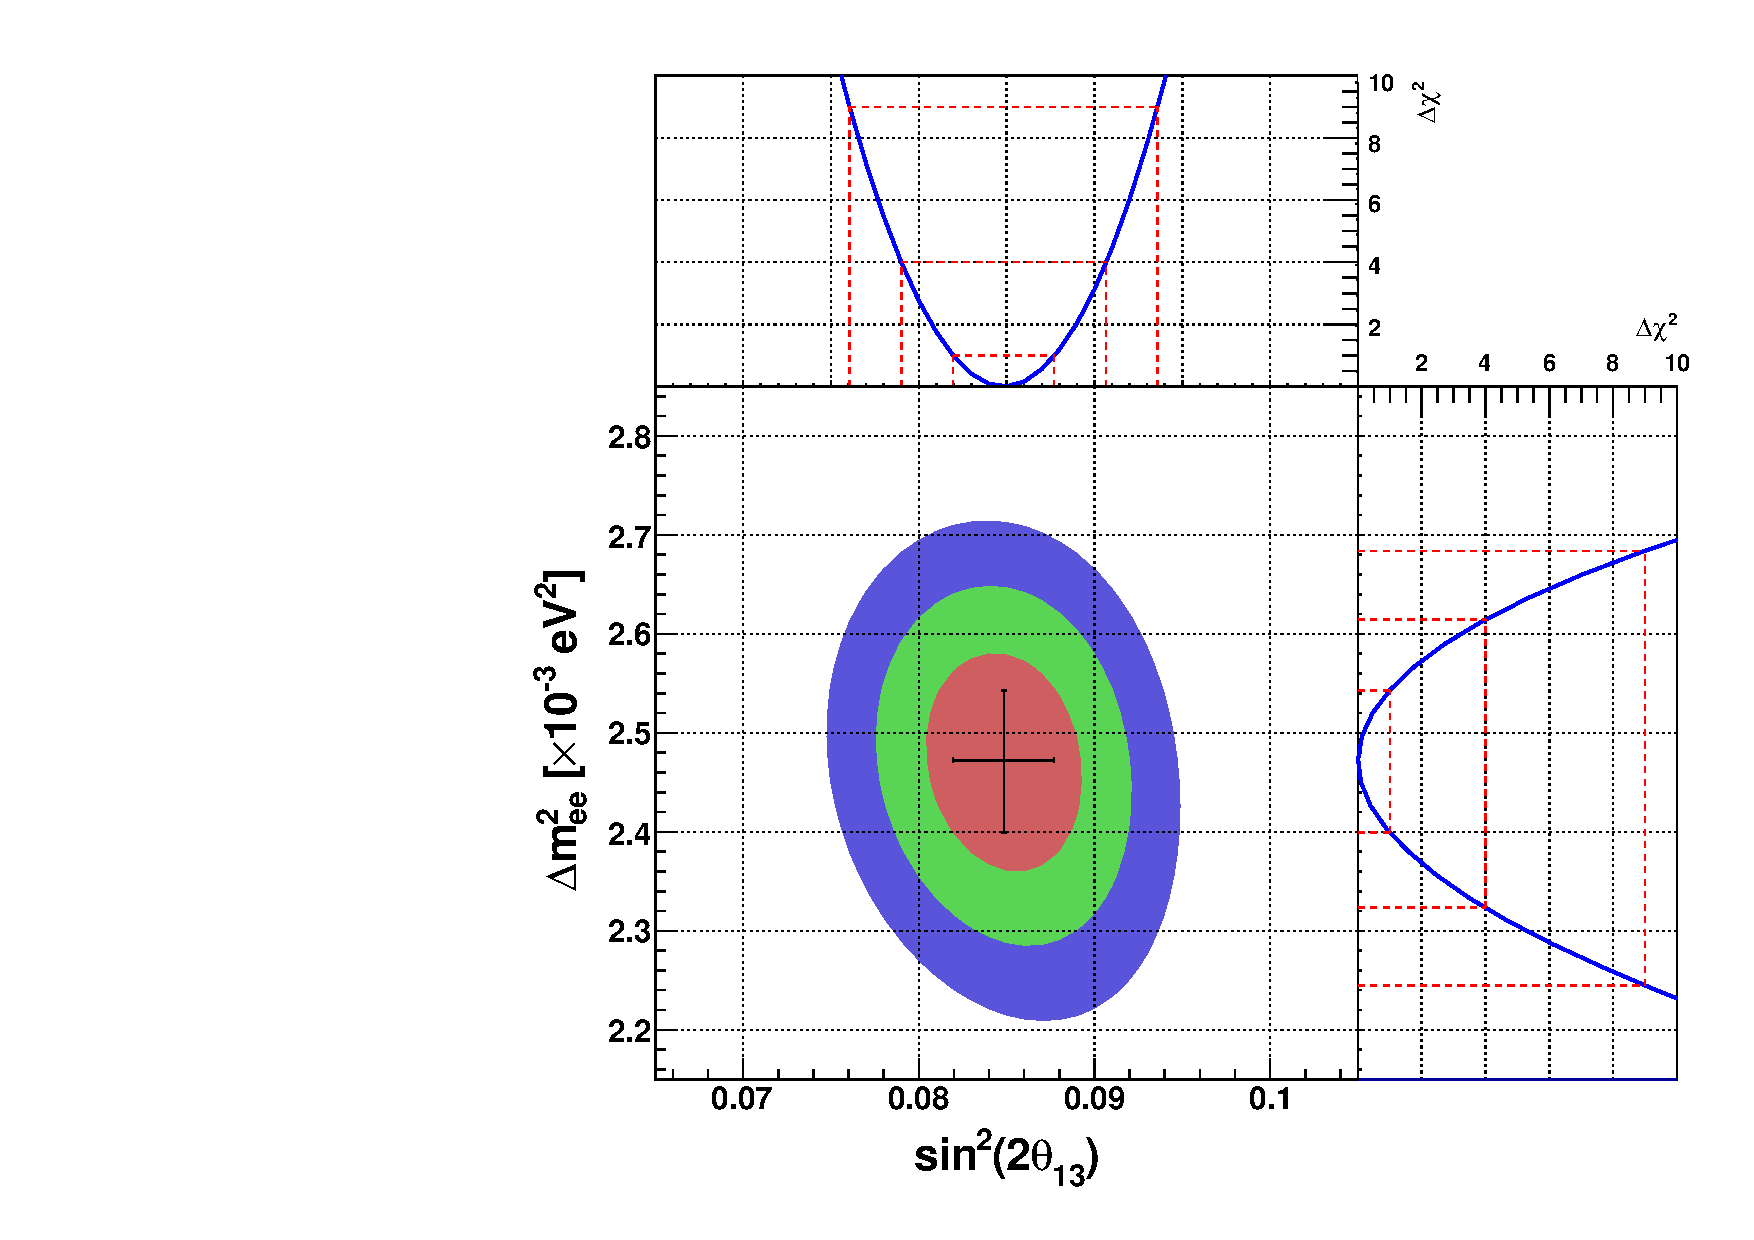
\includegraphics[scale=0.5]{Fitting/contour_Matt.pdf}
  \caption{68\%, 95\%, and 99\% C.L\@. contours obtained from running the fitter on our IBD sample. The black cross is the best-fit point.}
  \label{fig:fitContours}
\end{figure}

\end{document}
